\section{Flexibility in PSWare}
In this section, we discuss how PSWare can achieve the desired flexibility in different aspects of an event-based system, namely, event detection, event delivery and event subscription.

\subsection{Flexibility in Event Detection}
Event detection is the heart of an event-based system. However, different applications may have very different requirements on event detection. For example, many WSN-applications may want to minimize energy consumption to extend network life span. Fortunately, in PSWare, we can easily customize the event detection algorithm by using the middleware framework.

We demonstrate the flexibility in event detection through two examples in this subsection. The first example is TED \cite{lai:ted} which is an event detection algorithm that aims at minimizing energy consumption. The second example is 

The essential idea of TED is fusion point selection, where the sensor nodes detect events and select parent nodes according to the detection cost so that the cost for future event detection can be reduced.

%Need to use a new figure
\begin{figure}
\centering
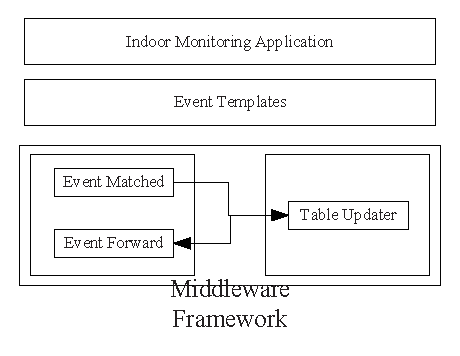
\includegraphics[width=.8\textwidth]{indoor-architecture}
\caption{TED over PSWare}
\label{fig:ted-architecture}
\end{figure}

\begin{algorithm}
\begin{algorithmic}
\REQUIRE \(v_n\rightarrow msg_r\)
	\FOR {each entry \(t'\) in \(msg_r\)}
		\IF {\NOT exists \(t'\rightarrow fid_n\) in \(table_r\)}
			\STATE \(addTo(table_r, t')\)
		\ENDIF
		\FOR {each entry \(t\) in \(table_r\)}
			\IF {\(t\rightarrow fid_n = t'\rightarrow f_n\)}
				\IF {\(t'\rightarrow hop_n < t\rightarrow hop_n\)}
					\STATE \(t\rightarrow hop_n \gets t\rightarrow hop_n+1\)
					\STATE \(t\rightarrow parent_n \gets v_n\)
				\ENDIF
			\ENDIF
		\ENDFOR
	\ENDFOR
	\IF {self is fusion point \AND \NOT exists \(self\rightarrow id\) in \(table_r\)}
		\STATE \(addTo(table_r, (self\rightarrow id, 0, self\rightarrow id))\)
	\ENDIF
	\STATE \(msg_r \gets table_r\)
	\STATE \(periodically\_broadcast(msg_r)\)
\end{algorithmic}
\caption{\(table_r\) construction}
\label{algo:table_r}
\end{algorithm}

In TED, we have a set of nodes \(V'\subseteq V\) selected as event fusion points. Each individual sensor nodes will maintain the following table \(table_r\) for all \(v'_n\in V'\)
\begin{itemize}
\item Fusion point ID (\(fid_n\)): the node ID of the fusion point:
\item	Hop count (\(hop_n\)): the number of hops to reach the fusion point
\item	Parent (\(parent_n\)): the next hop to that fusion point\\
\end{itemize}
Each sensor node will also maintain an event table \(table_e\) containing the information for each event type \(e_n\in E\) which includes the following fields:
\begin{itemize}
\item Event type ID (\(e_n\)): the ID which is assigned to each event type
\item Fusion point for the event (\(fusion_n\)): the fusion point at which the event is mostly likely to be detected at the lowest cost.
\item Fusion cost (\(cost_n\)): the fusion cost for event type \(e_n\)\\
\end{itemize}
In addition to the above tables, each fusion point \(v'\in V'\) will maintain another table \(table_m\) for the purpose of matching events. \(table_m\) contains the following fields:
\begin{itemize}
\item Event type ID (\(e_n\)): the ID of the event type
\item Event instance ID (\(i\)): the \(i\)th event instance of event type \(e_n\) (we use \(e_n^i\) to denote such an instance of event)
\item Source node (\(v_n^i\)): the node which forwarded \(e_n^i\) to the fusion point
\item Event timestamp (\(t_n^i\)): the timestamp when the event \(e_n^i\) is detected
\item Detection cost (\(cost_n^i\)): the cost for detecting event \(e_n^i\)
\end{itemize}

Each node \(v_n\) periodically broadcasts messages \(msg_r\) which is its \(table_r\). If the node itself is a fusion point, then it will add itself in \(table_r\) and broadcast the message. The procedure is shown in Procedure \ref{algo:table_r}.

In addition to \(msg_r\), each \(v'_k\in V'\) will periodically advertise its \(table_m\) by broadcasting \(msg_m\) so that other sensor nodes can construct their \(table_e\) with Procedure \ref{algo:table_e}.

\begin{algorithm}
\begin{algorithmic}
\REQUIRE \(v'_k\rightarrow msg_m\)
	\FOR {each entry \(t'\) in \(msg_m\)}
		\IF {\NOT exists \(t'\rightarrow e_n\) in \(table_e\)}
			\STATE \(addTo(table_e, (t'\rightarrow e_n, 1, v'_k, t'\rightarrow cost_n^i+table_r\rightarrow hop_k))\)
		\ENDIF
		\FOR {each entry \(t\) in \(table_e\)}
			\IF {\(t\rightarrow e_n = t'\rightarrow e_n\)}
				\IF {\(t'\rightarrow cost_n^i+table_r\rightarrow hop_k < t\rightarrow cost_n\)}
					\STATE \(t\rightarrow cost_n \gets t'\rightarrow cost_n^i+table_r\rightarrow hop_k\)
					\STATE \(t\rightarrow fusion_n \gets v'_k\)
				\ENDIF
			\ENDIF
		\ENDFOR
	\ENDFOR
	\IF {self is fusion point}
		\STATE \(msg_m \gets table_m\)
		\STATE \(periodically\_broadcast(msg_m)\)
	\ENDIF
\end{algorithmic}
\caption{\(table_e\) construction}
\label{algo:table_e}
\end{algorithm}

The construction of \(table_m\) will take place when the event instance \(e_n^i\) is detected and forwarded to a fusion point \(v'_n\). We will discuss how forwarding could be done in the next subsection.

When an event \(e_n^i\) is detected at node \(v_k\), node will use \(table_r\) and \(table_e\) to decide how to forward the detected event to the fusion points so that higher level events can be detected. The pseudo code is shown in Procedure \ref{algo:eventforwarding}.

\begin{algorithm}
\begin{algorithmic}
\REQUIRE detected event \(e_n^i\)
	\IF {\(table_e\rightarrow fusion_n=null\)}
		\STATE \(event\_forward(e_n^i)\)
	\ELSE
		\STATE \(send(e_n^i, table_e\rightarrow fusion_n)\)
	\ENDIF
\end{algorithmic}
\caption{Event forwarding}
\label{algo:eventforwarding}
\end{algorithm}

In case the fusion point for event type \(e_n\) has not been decided, the node will forward the event to some of its closet fusion points using the \(event\_forward\) function according to TED. Upon the reception of \(e_n^i\) from \(v_k\), the fusion point will first update its own \(table_m\). Then it will check if there is any composite event \(e_{comp}\) which uses \(e_n\) and another event \(e_j\) as its sub-event (\(e_{comp}=comp(e_n, e_j)\)). The pseudo code of event matching is shown in Procedure \ref{algo:eventmatching}.

\begin{algorithm}
\begin{algorithmic}
\REQUIRE \(e_n^i\) detected by \(v_k\) with cost: \(cost_n^i\)
	\STATE \(addTo(table_m, (e_n, e_n^i, v_k, now(), cost_n^i))\)
	\FOR {each \(e_j\) in \(E\)}
		\IF {\(\exists r\in R\) \AND \(r=e_{comp}=comp(e_n, e_j)\)}
			\FOR {each \(e_j^k\) in \(table_m\)}
				\IF {\(comp(e_n^i, e_j^k)=true\)}
					\STATE \(addTo(table_m, (e_{comp}, e_{comp}^i, self, now(), cost_n^i+cost_j^k))\)
					\STATE \(detected(e_{comp})\)
				\ENDIF
			\ENDFOR
		\ENDIF
	\ENDFOR
	\STATE \(event\_forward(e_n^i)\)
\end{algorithmic}
\caption{Event matching}
\label{algo:eventmatching}
\end{algorithm}

Note that if \(e_{comp}\) has been successfully detected, the procedure will run function \(detected\) which, in turn, will execute Procedure \ref{algo:eventforwarding}. The procedure will also use \(event\_forward\) in the end to forward the detected event to other fusion node so that better fusion point may be found.

Next 
\subsection{Flexibility in Event Delivery}

\subsection{Flexibility in Event Subscription}